\documentclass[class = article,border = 5pt]{standalone}

\usepackage[usenames,dvipsnames]{xcolor}

\usepackage{tikz}
\usetikzlibrary{arrows, shapes, fit, backgrounds, calc}

\usepackage{amsmath,amsfonts,amsthm,amssymb,mathtools}

\usepackage{/Users/kelly/Workspace/Utilities/luke-macros}

\pgfdeclarelayer{background}
\pgfsetlayers{background,main}

\setlength{\parskip}{0pt}
\setlength{\parindent}{0pt}

\begin{document}

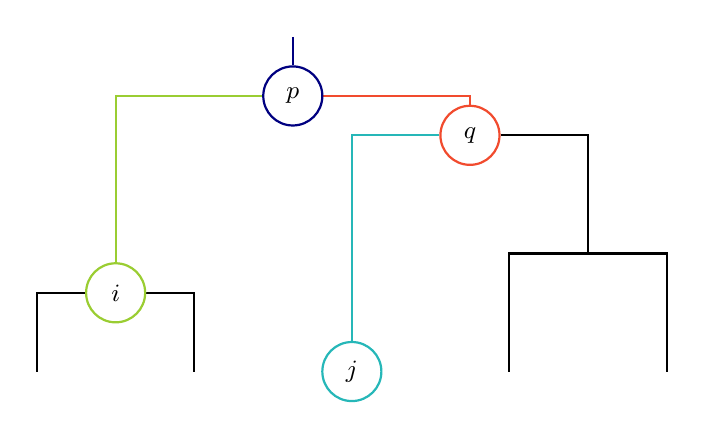
\begin{tikzpicture}

    % Sans-serif text
    \sffamily

    % Species tree
    \tikzset{nS/.style={draw, shape = circle, inner sep = 1pt, minimum width = 16pt}}
    \tikzset{inS/.style={nS, fill = white}}
    \tikzset{lnS/.style={nS, fill = black, text = white}}
    \tikzset{pS/.style={draw=black, thick}}

    % Labelled nodes
    \tikzset{Si/.style={thick, circle, inner sep = 0mm, minimum size = 0.75cm, font = \small, draw=YellowGreen}}
    \tikzset{Sp/.style={thick, circle, inner sep = 0mm, minimum size = 0.75cm, font = \small, draw=NavyBlue}}
    \tikzset{Sj/.style={thick, circle, inner sep = 0mm, minimum size = 0.75cm, font = \small, draw=BlueGreen}}
    \tikzset{Sq/.style={thick, circle, inner sep = 0mm, minimum size = 0.75cm, font = \small, draw=RedOrange}}

    % Labelled branches trees
    \tikzset{Bi/.style={thick, draw=YellowGreen}}
    \tikzset{Bp/.style={thick, draw=NavyBlue}}
    % \tikzset{Bsi/.style={thick, draw=Rhodamine}}
    \tikzset{Bj/.style={thick, draw=BlueGreen}}
    \tikzset{Bq/.style={thick, draw=RedOrange}}

    % Tree nodes
    \node (a) at (-1.75, 4.25) {};
    	\node (p) [Sp] at (-1.75, 3.5) {$ p $};
    		\node (i) [Si] at (-4, 1) {$ i $ };
                \node (oi1) at (-5, 0) {};
                \node (oi2) at  (-3, 0) {};
    		\node (q) [Sq] at (0.5, 3) {$ q $};
    			\node (oj) at (2, 1.5) {};
    				\node (oj1) at (1, 0) {};
    				\node (oj2) at (3, 0) {};
    			\node (j) [Sj] at (-1, 0) {$ j $};

    % Background image
    \begin{pgfonlayer}{background}

    	% Species tree
    	\path[Bp] (a.center) -- (p);
    		\path[Bi] (p) -| (i);
                \path[pS] (i) -| (oi1.center);
                \path[pS] (i) -| (oi2.center);
    		\path[Bq] (p) -| (q);
    			\path[pS] (q) -| (oj.center);
    				\path[pS] (oj.center) -| (oj1.center);
    				\path[pS] (oj.center) -| (oj2.center);
    			\path[Bj] (q) -| (j);

    \end{pgfonlayer}

\end{tikzpicture}

\begin{tikzpicture}

    \node [white] at (0, 0) {~};
    \node [white] at (0, 4.25) {~};
    \draw[red, thick, ->, >= triangle 60] (-1, 2.5) -- (1, 2.5);

\end{tikzpicture}

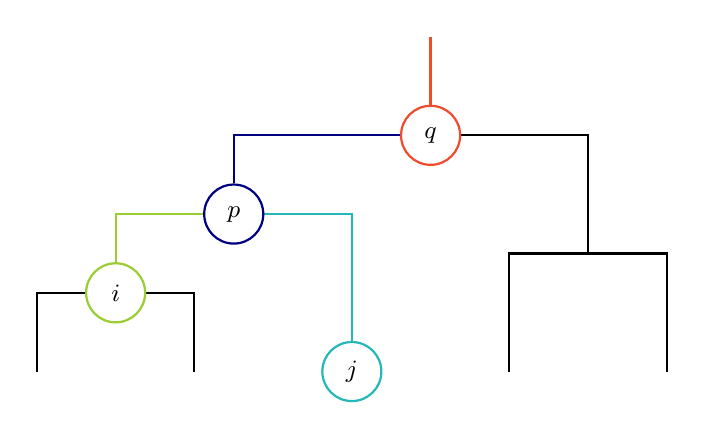
\begin{tikzpicture}

    % Sans-serif text
    \sffamily

    % Species tree
    \tikzset{nS/.style={draw, shape = circle, inner sep = 1pt, minimum width = 16pt}}
    \tikzset{inS/.style={nS, fill = white}}
    \tikzset{lnS/.style={nS, fill = black, text = white}}
    \tikzset{pS/.style={draw=black, thick}}

    % Labelled nodes
    \tikzset{Si/.style={thick, circle, inner sep = 0mm, minimum size = 0.75cm, font = \small, draw=YellowGreen}}
    \tikzset{Sp/.style={thick, circle, inner sep = 0mm, minimum size = 0.75cm, font = \small, draw=NavyBlue}}
    \tikzset{Sj/.style={thick, circle, inner sep = 0mm, minimum size = 0.75cm, font = \small, draw=BlueGreen}}
    \tikzset{Sq/.style={thick, circle, inner sep = 0mm, minimum size = 0.75cm, font = \small, draw=RedOrange}}

    % Labelled branches trees
    \tikzset{Bi/.style={thick, draw=YellowGreen}}
    \tikzset{Bp/.style={thick, draw=NavyBlue}}
    % \tikzset{Bsi/.style={thick, draw=Rhodamine}}
    \tikzset{Bj/.style={thick, draw=BlueGreen}}
    \tikzset{Bq/.style={thick, draw=RedOrange}}

    % Tree nodes
    \node (a) at (0, 4.25) {};
    	\node (q) [Sq] at (0, 3) {$ q $};
    		\node (p) [Sp] at (-2.5, 2) {$ p $};
    			\node (i) [Si] at (-4, 1) {$ i $ };
                    \node (oi1) at (-5, 0) {};
                    \node (oi2) at  (-3, 0) {};
    			\node (j) [Sj] at (-1, 0) {$ j $};
    		\node (oj) at (2, 1.5) {};
    			\node (oj1) at (1, 0) {};
    			\node (oj2) at (3, 0) {};

    % Background image
    \begin{pgfonlayer}{background}

    	% Species tree
    	\path[Bq] (a.center) -- (q);
    		\path[Bp] (q) -| (p);
    			\path[Bi] (p) -| (i);
                    \path[pS] (i) -| (oi1.center);
                    \path[pS] (i) -| (oi2.center);
    			\path[Bj] (p) -| (j);
    		\path[pS] (q) -| (oj.center);
    			\path[pS] (oj.center) -| (oj1.center);
    			\path[pS] (oj.center) -| (oj2.center);

    \end{pgfonlayer}

    \end{tikzpicture}

\end{document}
